%-------------------------------------------------------------------------------
% Methoden
%-------------------------------------------------------------------------------
\section{Ergebnisse}
Nachfolgend erfolgt die Untersuchung der Ergebnisse des Experiments.

\subsection{Beschreibung der Stichprobe}\label{beschreibung}
Die Studie startete am 05.07.2020 und endete am 14.09.2020. Das Experiment war für die gesamte Dauer der Studie durchgehend erreichbar. In diesem Zeitraum nahmen 279 Teilnehmer an dem Experiment teil. Zunächst wurden 13 Einträge aus dem Datensatz entfernt, die in der folgenden Auswertung nicht berücksichtigt werden. Bei diesen Einträgen handelt es sich um Mehrfachteilnahmen, die sich durch eine identische IP-Adresse sowie identische User-Agents auszeichneten. Es wurde in diesem Fall lediglich die erstmalige Teilnahme berücksichtigt. Sämtliche nachfolgenden Einträge wurde aus dem Datensatz eliminiert. Zusätzlich wurden Einträge gelöscht, bei denen der Proband keinen Befehl abgeschickt hat. Damit hat der bereinigte Datensatz einen Umfang von 244 Teilnehmern. Davon haben 18 Personen das Experiment vollständig durchlaufen und sämtliche Fragen korrekt beantwortet.

Von den verbleibenden Versuchspersonen gaben 81.1 \% der Teilnehmer an, männlich zu sein. 9.1 \% gaben ein weibliches Geschlecht und 9.9 \% ein anderes Geschlecht an. Der Großteil der Teilnehmer gab an, über sehr gute (43.4 \%) oder gute (41.8 \%) Englischkenntnisse zu verfügen. Lediglich 9.0 \% verfügten über schlechte Kenntnisse und 5.7 \% verfügten über keinerlei englische Sprachkenntnisse. Die Altersverteilung der Versuchspersonen ist wie folgt: 38.1 \% gaben 18-29 Jahre an, 35.7 \%  29-39 Jahre,  15.6 \% 39-59 Jahre, 4.9 \% weniger als 18 Jahre und 5.7 \% gaben an, älter als 59 Jahre zu sein. Damit waren zum Zeitpunkt des Experiments 89.3 \% der Teilnehmer zwischen 18 und 59 Jahre alt. Davon nutzt ein Großteil die Kommandozeile mindestens einmal im Monat (47.5 \% täglich, 24.2 \% wöchentlich, 9.4 \% monatlich). Demgegenüber nutzen 11.1 \% die Kommandozeile selten (1x im Jahr oder weniger) oder gar nicht (7.8 \%). Damit setzt sich die Stichprobe aus überwiegend jungen Versuchspersonen, die über gute Englischkenntnisse verfügen und bereits erste Erfahrungen mit der Kommandozeile haben, zusammen.

\subsection{Deskriptive Statistik}

\begin{figure}[htbp]
    \centering
    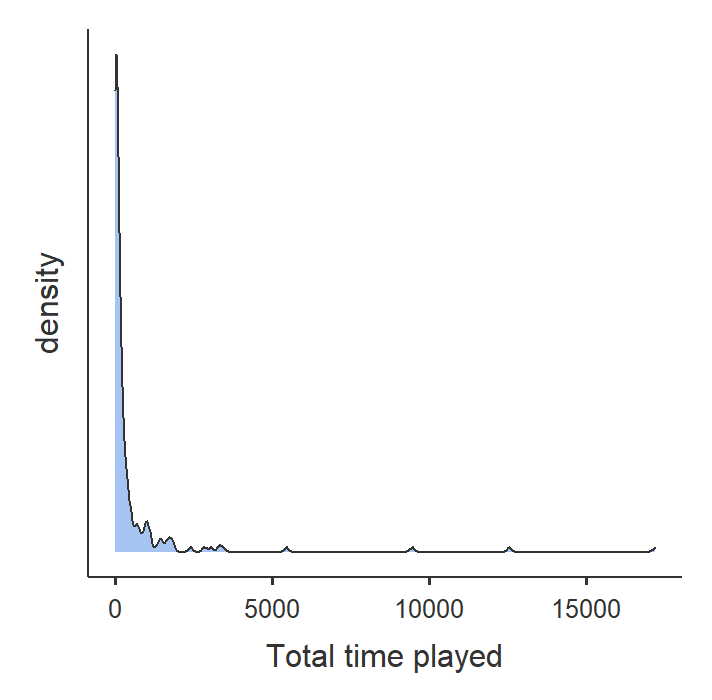
\includegraphics[width=0.5\textwidth]{img/auswertung/density.png}
    \caption{Die Verteilungskurve aller Teilnehmer hinsichtlich der Gesamtspielzeit.}
    \label{density}
\end{figure}

Im Mittel verbrachten die Teilnehmer 8 Minuten und 46 Sekunden (527 Sekunden, $SD = 1588$ Sekunden) mit dem Experiment und setzten dabei durchschnittlich 19.5 Befehle ab (SD= 23.0). Sowohl bei der Gesamtdauer als auch bei der Anzahl der abgesendeten Befehle gibt es extreme Ausreißer nach oben. So investierte ein Teilnehmer fast 5 Stunden in das Experiment und verwendete dabei 84 unterschiedliche Befehle. Diese enorme Streuung nach oben wird auch in Abbildung \ref{density} deutlich. Aus diesem Grund wird nachfolgend zusätzlich der Median betrachtet, da dieser robuster gegenüber Ausreißern ist.

% Anzahl Befehle
\begin{figure}[htbp]
    \centering
    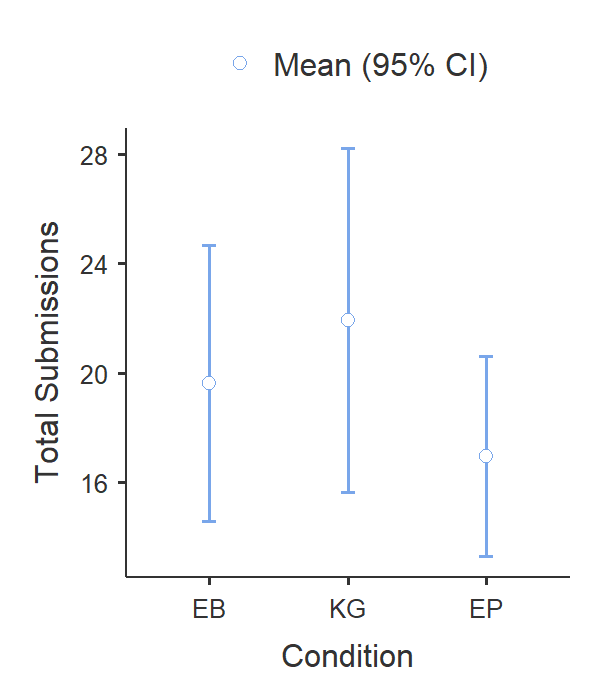
\includegraphics[width=0.5\textwidth]{img/auswertung/mean_subs.png}
    \caption{Mittelwerte für die Gesamtzahl abgesetzter Befehle. EB= Experimentalbedingung Abzeichen, KG= Kontrollgruppe und EP = Experimentalbedingung Fortschrittsanzeige.}
    \label{mean_subs}
\end{figure}

Im Mittel nutzen Teilnehmer der Kontrollgruppe mit 21.9 Befehlen die meisten Kommandos ($SD = 27.3$). Die Versuchsbedingung 'Abzeichen' weist im Vergleich eine durchschnittliche Anzahl abgesetzter Befehle von 19.6 (SD = 24.1) auf, während es Probanden aus der Bedingung 'Fortschrittsanzeige' auf durchschnittlich 16.9 Befehle bringen ($SD=16.3$). Die Mittelwerte sind in Abbildung \ref{mean_subs} dargestellt. Hier fällt erneut das breite Streuungsintervall auf. Betrachtet man stattdessen den Median der einzelnen Versuchsbedingungen, bleibt die Kontrollgruppe mit 13 Kommandos pro Teilnehmer die aktivste Bedingung. Allerdings sind Probanden der Experimentalgruppe 'Fortschrittsanzeige' im Median ($\tilde x = 11$ Befehle) aktiver als Teilnehmer, die ein Abzeichen erhielten ($\tilde x = 9$ Befehle). Der Median der erfolgreich gelösten Aufgaben liegt im Fall der Experimentalbedingungen bei 3 Aufgaben und bei der Versuchsbedingung bei 4.

% Investierte Zeit
\begin{figure}[htbp]
    \centering
    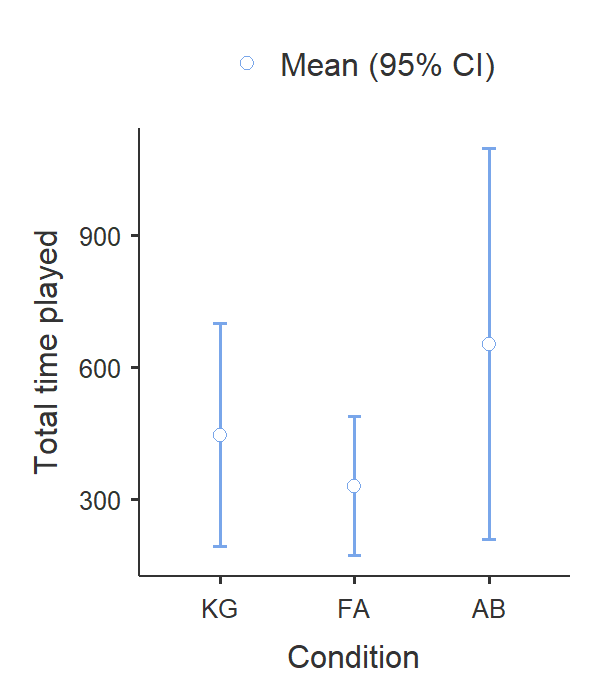
\includegraphics[width=0.5\textwidth]{img/auswertung/mean_time.png}
    \caption{Mittelwerte für die Gesamtzeit, die die Teilnehmer in das Experiment investierten. EB= Experimentalbedingung Abzeichen, KG= Kontrollgruppe und EP = Experimentalbedingung Fortschrittsanzeige.}
    \label{mean_time}
\end{figure}

Betrachtet man die Zeit, die die Teilnehmer im Mittel in das Experiment investiert haben, fällt auf, dass die Teilnehmer der Versuchsbedingung 'Abzeichen' mit 797 Sekunden (SD= 2256 Sekunden) deutlich mehr Zeit als die Kontrollgruppe (	$\bar{x} = 495$ Sekunden; SD = 1212 Sekunden) investierten. Letztere hat wiederum mehr Zeit investiert, als die Probanden der Versuchsbedingung 'Fortschrittsanzeige'. Diese brachten es auf vergleichsweise kurze 364 Sekunden (SD= 769 Sekunden). Die entsprechenden Mittelwerte sind in Abbildung \ref{mean_time} dargestellt. Betrachtet man auch hier den Median und nicht die Mittelwerte, ändert sich das Ergebnis deutlich. Die jeweiligen Mediane der unterschiedlichen Bedingungen liegen deutlich näher beieinander. So bringen es Teilnehmer der Bedingung 'Abzeichen' auf 149 Sekunden (~2.5 Minuten) und bringen damit ähnlich viel Zeit für das Experiment wie die Probanden der Kontrollgruppe (154 Sekunden) auf. Etwas weniger Zeit wurde im Durchschnitt von Teilnehmern investiert, die eine Fortschrittsanzeige angezeigt bekamen ($\tilde x = 132$ Sekunden).

Aufgrund der hohen Diskrepanz zwischen Median und Mittelwert sowie der extrem hohen Standardabweichung habe ich beschlossen, extreme Ausreißer aus der weiteren Betrachtung auszuschließen. Bei diesen Ausreißern gehe ich davon aus, dass eine, von den Spielelementen unabhängige, Intrinsische Motivation vorliegt. Als Grenzwert wählte ich $\pm 2\sigma$. Dies führt dazu, dass sämtliche Teilnehmer mit mehr als 3703 Sekunden Spieldauer aus dem Datensatz ausgeschlossen werden. Damit reduziert sich der Datensatz im Folgenden auf einen Umfang von 240 Probanden.

\subsection{Hypothesenüberprüfung}
Die aufgestellten Hypothesen werden durch einen t-Test und eine einfaktorielle  ANOVA  Varianzanalyse überprüft. Zunächst sind die Voraussetzungen Normalverteilung und Varianzhomogenität zu prüfen. Da jede Versuchsbedingung einen Umfang von deutlich über 30 Probanden aufweist, kann von einer Normalverteilung ausgegangen werden. Um die Vorraussetzung der Varianzhomogenität zu prüfen, habe ich einen Levene-Test durchgeführt. Bei diesem handelt es sich um einen Signifikanztest. Dieser prüft, ob die Varianzen innerhalb von zwei oder mehr Grundgesamtheiten (Gruppen) gleich sind (H0). Daraus ergibt sich die Alternativhypothese (H1), dass mindestens ein Gruppenpaar ungleiche Varianzen besitzt. Befindet sich der p-Wert unterhalb  eines zuvor definierten Signifikanzniveaus sind die Unterschiede in den Varianzen der unterschiedlichen Stichproben signifikant. Folglich kann die Nullhypothese des Tests abgelehnt werden. Für den Test gehe ich von einem Signifikanzniveau von 5\% aus. 

\subsubsection{Überprüfung mittels t-Test}

\paragraph{Hypothese 1 }
\begin{center}
    \textit{Probanden, die Abzeichen erhalten (EB), beantworten im Mittel eine höhere Anzahl an Fragen als eine Kontrollgruppe ohne Abzeichen (KG).} 
\end{center}

Die Differenz der durchschnittlichen Anzahl beantworteter Fragen von Probanden der Experimentalbedingung 'Abzeichen' ($M =4.04;\:SD=3.20$) und Probanden der Kontrollgruppe ohne Spielelemente ($M=4.30;\:SD=3.86$) war nicht signifikant ($t (124) = -0.40451;\: p = 0.657$). Die Hypothese konnte damit nicht bestätigt werden. Aus diesem Grund wandelte ich die ursprüngliche Hypothese ab, um ein tiefergehendes Verständnis der Daten zu erlangen: 

\begin{itemize}
    \item \textbf{1.A:} \textit{Probanden, die Abzeichen erhalten, verbringen im Mittel mehr Zeit mit dem Experiment als eine Kontrollgruppe ohne Spielelemente.}
    \item \textbf{1.B:} \textit{Probanden, die Abzeichen erhalten, benutzen durchschnittlich mehr Befehle als eine Kontrollgruppe ohne Spielemente.} 
\end{itemize}

Die Ergebnisse für den t-Test sind in Tabelle \ref{ttest_hypo_1} dargestellt. Der p-Wert blieb für beide Hypothesen deutlich oberhalb des Signifikanzniveaus. Folglich müssen beiden Hypothesen abgelehnt werden. Bei allen drei Hypothesen war die Signifikanz des Levene-Tests oberbahlb des üblichen Grenzwertes von 0.05. Damit kann angenommen werden, dass die Varianzen der beiden Stichproben gleich sind. Entsprechend sind die Voraussetzungen für die Durchführung eines t-Tests erfüllt.

% ~*~*~*~*~*~*~*~*~*~*~*~*~*~*~*~ LEVENE - HYPO 1 ~*~*~*~*~*~*~*~*~*~*~*~*~*~*~*~
\begin{table}[htbp]
\centering
\begin{tabular}{ |p{4cm}||p{2.0cm}|p{2.0cm}|p{2.0cm}|p{2.0cm}| }
 \hline
 \multicolumn{5}{|c|}{Test auf Varianzhomogenität (Levene's)} \\
 \hline
 & F & df1 &df2 &p \\
 \hline
  Befehlanzahl      & 0.0227    & 1 &   124 & 0.880\\
  Gesamtspielzeit   & 0.0284    & 1 &   124 & 0.867\\
  Gelöste Aufgaben  & 1.9587    & 1 &   124 & 0.164\\
 \hline
\end{tabular}
\caption{Levene-Test auf Varianzhomogenität für die Experimentalbedingung Abzeichen (Hypothese 1). Auf dem 5\%-Niveau signifikante p-Werte sind durch ein * gekennzeichnet}
\label{levene_hypo_1}
\end{table}
% ~*~*~*~*~*~*~*~*~*~*~*~*~*~*~*~ END ~*~*~*~*~*~*~*~*~*~*~*~*~*~*~*~
% ~*~*~*~*~*~*~*~*~*~*~*~*~*~*~*~ TEST - HYPO 1 ~*~*~*~*~*~*~*~*~*~*~*~*~*~*~*~
\begin{table}[htbp]
\centering
\begin{tabular}{ |p{4cm}||p{2.0cm}|p{2.0cm}|p{2.0cm}| }
 \hline
 \multicolumn{4}{|c|}{Zweistichproben-t-Test (Students's t)} \\
 \hline
 & T &df & p \\
 \hline
  Befehlanzahl       & 0.16608  &   124 & 0.434\\
  Gesamtspielzeit    & -0.00332 &   124 & 0.501\\
  Gelöste Aufgaben   & -0.40451 &   124 & 0.657\\
 \hline
\end{tabular}
\caption{Zweistichproben-t-Test für die Experimentalbedingung Abzeichen und Kontrollgruppe (Hypothese 1). Anmerkung: $H_a:\: EB > KG$}
\label{ttest_hypo_1}
\end{table}
% ~*~*~*~*~*~*~*~*~*~*~*~*~*~*~*~ END ~*~*~*~*~*~*~*~*~*~*~*~*~*~*~*~



\paragraph{Hypothese 2 }
\begin{center}
    \textit{Probanden, die eine Fortschrittsanzeige erhalten (EP), beantworten im Mittel eine höhere Anzahl an Fragen als eine Kontrollgruppe ohne Fortschrittsanzeige (KG).} 
\end{center}

Die Differenz der durchschnittlichen Anzahl beantworteter Fragen von Probanden der Experimentalbedingung 'Fortschrittsanzeige' ($M =4.30;\:SD=3.86$) und Probanden der Kontrollgruppe ($M=4.27;\:SD=3.65$) war nicht signifikant ($t (116) = 0.0443;\: p = 0.482$). Auch diese Hypothese konnte damit nicht bestätigt werden. Die für Hypothese 1 abgewandelten Hypothesen wurden auch für die Versuchsbedingung 'Fortschrittsanzeige' aufgestellt: 

\begin{itemize}
    \item \textbf{1.A:} \textit{Probanden, die eine Fortschrittsanzeige erhalten, verbringen im Mittel mehr Zeit mit dem Experiment als eine Kontrollgruppe ohne Spielelemente.}
    \item \textbf{1.B:} \textit{Probanden, die eine Fortschrittsanzeige erhalten, benutzen durchschnittlich mehr Befehle als eine Kontrollgruppe ohne Spielelemente.} 
\end{itemize}

Die Ergebnisse für die Hypothesen sind in Tabelle \ref{levene_hypo_2} dargestellt. Erneut ist kein Test signifikant und folglich kann keine Hypothese bestätigt werden. Zwei Beobachtungen sind dabei besonders auffällig: Zum einen fällt ein großer Unterschied in der mittleren Spielzeit und der Anzahl benutzter Befehle auf. Insbesondere die Spielzeit unterscheidet sich zwischen der Experimentalbedingung ($M=255.03$) deutlich von der Kontrollgruppe ($M=382.04$). Dieser Unterschied spiegelt sich auch im t-Test wieder ($t(116)=1.2056$). Mit einem p-Wert von $p=0.115$ ist der Test zwar nicht signifikant, jedoch im Vergleich zu den anderen Ergebnissen deutlich reduziert. Damit kann von einem gegenteiligen Effekt ausgegangen werden, als ursprünglich antizipiert. Die Fortschrittsanzeige scheint sich tendenziell negativ auf das Durchhaltevermögen der Teilnehmer auszuwirken. Auffällig ist zudem der signifikante p-Wert ($p=0.030$) des Levene-Tests für die Gesamtspielzeit. Dies deutet auf eine Verletzung der Annahme von Varianzhomogenität hin. Damit ist zwar die Voraussetzung für die Durchführung des t-Tests formal nicht erfüllt, jedoch ist der t-Test sehr robust gegenüber Verletzungen seiner Voraussetzungen. Aus diesem Grund werden die Ergebnisse trotzdem berücksichtigt.

% ~*~*~*~*~*~*~*~*~*~*~*~*~*~*~*~ LEVENE - HYPO 2 ~*~*~*~*~*~*~*~*~*~*~*~*~*~*~*~
\begin{table}[htbp]
\centering
\begin{tabular}{ |p{4cm}||p{2.0cm}|p{2.0cm}|p{2.0cm}|p{2.0cm}| }
 \hline
 \multicolumn{5}{|c|}{Test auf Varianzhomogenität (Levene's)} \\
 \hline
 & F & df1 &df2 &p \\
 \hline
  Befehlanzahl      & 2.902     & 1 &   116 & 0.091\\
  Gesamtspielzeit   & 4.814     & 1 &   116 & 0.030*\\
  Gelöste Aufgaben  & 0.190     & 1 &   116 & 0.664\\
 \hline
\end{tabular}
\caption{Levene-Test auf Varianzhomogenität für die Experimentalbedingung Fortschrittsanzeige (Hypothese 2). Auf dem 5\%-Niveau signifikante p-Werte sind durch ein * gekennzeichnet}
\label{levene_hypo_2}
\end{table}
% ~*~*~*~*~*~*~*~*~*~*~*~*~*~*~*~ END ~*~*~*~*~*~*~*~*~*~*~*~*~*~*~*~
% ~*~*~*~*~*~*~*~*~*~*~*~*~*~*~*~ TEST - HYPO 2 ~*~*~*~*~*~*~*~*~*~*~*~*~*~*~*~
\begin{table}[htbp]
\centering
\begin{tabular}{ |p{4cm}||p{2.0cm}|p{2.0cm}|p{2.0cm}| }
 \hline
 \multicolumn{4}{|c|}{Zweistichproben-t-Test (Students's t)} \\
 \hline
 & T &df & p \\
 \hline
  Befehlanzahl       & 0.7447   &   116 & 0.229\\
  Gesamtspielzeit    & 1.2056   &   116 & 0.115\\
  Gelöste Aufgaben   & 0.0443   &   116 & 0.482\\
 \hline
\end{tabular}
\caption{Zweistichproben-t-Test für die Experimentalbedingung Abzeichen und Kontrollgruppe (Hypothese 1). Anmerkung: $H_a:\: EP > KG$}
\label{ttest_hypo_2}
\end{table}
% ~*~*~*~*~*~*~*~*~*~*~*~*~*~*~*~ END ~*~*~*~*~*~*~*~*~*~*~*~*~*~*~*~

% ~*~*~*~*~*~*~*~*~*~*~*~*~*~*~*~ ANOVA ~*~*~*~*~*~*~*~*~*~*~*~*~*~*~*~
\subsubsection{Überprüfung mittels ANOVA Varianzanalyse }
Bei der ANOVA (engl. \textit{Analysis of Variance}) handelt es sich um eine Varianzanalyse, die die Mittelwerte von mehr als 2 Gruppen vergleichbar macht. Dabei handelt es sich um eine Erweiterung des t-Tests, welcher auf den Vergleich von maximal 2 Stichproben beschenkt ist. Nachfolgend werden die zwei abhängigen Variablen \textbf{Gelöste Aufgaben} und \textbf{Gesamtspielzeit} jeweils durch eine einfaktorielle Varianzanalyse untersucht.

% Varianzhomogenität prüfen 
Zunächst gilt es erneut die Voraussetzung der Varianzhomogenität mittels Levene-Test zu prüfen. Wie in Tabelle \ref{levene_amova} zu sehen, ist die Signifikanz der Zeile \textit{Gesamtspielzeit} mit $p=0.048$ knapp unterhalb des Signifikanzniveaus von 5\%. Damit ist die Voraussetzung für die Durchführung einer ANOVA formal nicht gegeben. Aufgrund der minimalen Unterschreitung des Grenzwertes ($\Delta=0.002$) habe ich entschlossen, die Analyse dennoch durchzuführen. Ich nehme daher an, dass die Varianzen in den verschiedenen Stichproben gleich sind.

% ~*~*~*~*~*~*~*~*~*~*~*~*~*~*~*~ LEVENE - ANOVA ~*~*~*~*~*~*~*~*~*~*~*~*~*~*~*~
\begin{table}[htbp]
\centering
\begin{tabular}{ |p{4cm}||p{2.0cm}|p{2.0cm}|p{2.0cm}|p{2.0cm}| }
 \hline
 \multicolumn{5}{|c|}{Test auf Varianzhomogenität (Levene's)} \\
 \hline
 & F & df1 &df2 &p \\
 \hline
  Gelöste Aufgaben      & 1.01     & 1 &   187 & 0.365\\
  Gesamtspielzeit       & 3.09     & 1 &   187 & 0.048*\\
 \hline
\end{tabular}
\caption{Levene-Test auf Varianzhomogenität. Auf dem 5\%-Niveau signifikante p-Werte sind durch ein * gekennzeichnet}
\label{levene_amova}
\end{table}
% ~*~*~*~*~*~*~*~*~*~*~*~*~*~*~*~ END ~*~*~*~*~*~*~*~*~*~*~*~*~*~*~*~

Mit $F(2,187) = 1.02$ und einer Signifikanz von $p=0.903$ gibt es keinen statisch signifikanten Unterschied der Gruppenmittelwerte hinsichtlich der Anzahl gelöster Aufgaben. Ein ähnliches Ergebnis liefert die ANOVA für die Gesamtspielzeit ($F=0.967$). Allerdings ist dieses Resultat mit $p=0.382$ deutlich signifikanter, auch wenn es sehr deutlich oberhalb dem Signifikanzniveau liegt. Damit kann gezeigt werden, dass kein signifikanter Unterschied im Zusammenhang der Anzahl gelöster Aufgaben sowie der Gesamtspielzeit zwischen den Teilnehmern besteht, die unterschiedliche Spielelemente erhalten haben.

Obwohl die Werte der einzelnen Gruppen sich nicht signifikant voneinander unterscheiden, habe ich einen Post-hoc Test durchgeführt, um tiefer gehende Einblicke in die Daten zu erlangen. Ich verwendete dazu einen Tukey Test, da gleiche Varianzen vorliegen. Die Ergebnisse sind in Tabelle \ref{tukey_subs} (Befehle) und Tabelle \ref{tukey_time} (Gesamtspielzeit) dargestellt. Erwartungsgemäß findet sich kein signifikanter p-Wert. Dies ist in Anbetracht der nicht festgestellten Signifikanz in der ANOVA wenig verwunderlich. Es finden sich jedoch zwei Auffälligkeiten: 

Zunächst fallen die vergleichsweise hohen p-Werte ($p \in \{ 0.916, 0.928, 0.999, 1.000\}$) auf. Dies deutet darauf hin, dass sich die einzelnen Stichproben kaum bis gar nicht voneinander unterscheiden. Dies wird besonders für die Anzahl der gelösten Aufgaben deutlich (siehe Tabelle \ref{tukey_subs}). Auch unterscheiden sich die Experimentalbedingung 'Abzeichen' und die Kontrollgruppe hinsichtlich der Gesamtspielzeit nahezu überhaupt nicht ($p\approx1$). Darüber hinaus ist die mittlere Abweichung der Gesamtspielzeit zwischen den Experimentalbedingungen 'Abzeichen' und 'Fortschrittsanzeige' auffällig. Probanden, die eine Fortschrittsanzeige sahen, verbrachten im Mittel \nicefrac{1}{3} weniger Zeit mit dem Experiment (MD=127) als Teilnehmer, die Abzeichen erhielten, bzw. als Teilnehmer, die gar kein Spielelement erhielten.

% ~*~*~*~*~*~*~*~*~*~*~*~*~*~*~*~ POSTHOC ~*~*~*~*~*~*~*~*~*~*~*~*~*~*~*~


\begin{table}[htbp]
\centering
\begin{tabular}{ p{2cm} p{4cm} p{2.0cm} p{2.0cm} p{2.0cm} }
 \hline
 \multicolumn{5}{c}{Tukey Post-Hoc Test} \\
 \hline
 & & EB & KG & EP \\
 \hline
  EB    &   Mittlere Abweichung     & -     & -0.255        & -0.2240          \\
        &   t                       & -     & -0.398        & -0.3672          \\
        &   df                      & -     & 187           & 187              \\
        &   p                       & -     & \fbox{0.916}  & \fbox{0.928}     \\
  & & & &\\
  KG    &   Mittlere Abweichung     &       & -    & 0.0307         \\
        &   t                       &       & -    & 0.0468         \\
        &   df                      &       & -    & 187            \\
        &   p                       &       & -    & \fbox{0.999}          \\
  & & & &\\
  EP    &   Mittlere Abweichung     &       &       & - \\
        &   t                       &       &       & - \\
        &   df                      &       &       & - \\
        &   p                       &       &       & - \\
  
 \hline
\end{tabular}
\caption{Tukey Post-Hoc Test für die Gruppen Experimentalbedingung Abzeichen (EB), Experimentalbedingung Fortschrittsbalken (EP) und Kontrollgruppe (KG). Abhängige Variable: \textbf{Anzahl gelöster Aufgaben}}
\label{tukey_subs}
\end{table}


\begin{table}[htbp]
\centering
\begin{tabular}{ p{2cm} p{4cm} p{2.0cm} p{2.0cm} p{2.0cm} }
 \hline
 \multicolumn{5}{c}{Tukey Post-Hoc Test} \\
 \hline
 & & EB & KG & EP \\
 \hline
  EB    &   Mittlere Abweichung     & -     & -0.384    & \fbox{127}   \\
        &   t                       & -     & -0.00359  & 1.24         \\
        &   df                      & -     & 187       & 187          \\
        &   p                       & -     & \fbox{1.000}     & 0.431 \\
  & & & &\\
  KG    &   Mittlere Abweichung     &       & -         & 127   \\
        &   t                       &       & -         & 1.16  \\
        &   df                      &       & -         & 187   \\
        &   p                       &       & -         & 0.480 \\
  & & & &\\
  EP    &   Mittlere Abweichung     &       &           & -     \\
        &   t                       &       &           & -     \\
        &   df                      &       &           & -     \\
        &   p                       &       &           & -     \\
  
 \hline
\end{tabular}
\caption{Tukey Post-Hoc Test für die Gruppen Experimentalbedingung Abzeichen (EB), Experimentalbedingung Fortschrittsbalken (EP) und Kontrollgruppe (KG). Abhängige Variable: \textbf{Gesamtspielzeit}}
\label{tukey_time}
\end{table}

% ~*~*~*~*~*~*~*~*~*~*~*~*~*~*~*~ POSTHOC - END ~*~*~*~*~*~*~*~*~*~*~*~*~*~*~*~

\subsection{Zwischenfazit t-Test und ANOVA}
Die geschilderten Ergebnisse entsprechen nicht meinen ursprünglichen Erwartungen. Tatsächlich kann weder durch einen t-Test noch durch eine ANOVA ein signifikanter Effekt auf die Anzahl gelöster Aufgaben, die Menge der abgesetzten Befehle oder die Gesamtspielzeit nachgewiesen werden. Als Konsequenz kann keine meiner ursprünglich aufgestellten Hypothesen bestätigt werden. Die Spielelemente Abzeichen und Fortschrittsbalken zeigen damit in meinem Experiment keinerlei statisch signifikanten, positiven Effekt auf das Durchhaltevermögen (gemessen durch die Gesamtspielzeit) der Teilnehmer. Auch lässt sich keine erhöhte Aktivität der Probanden feststellen, da sich die Versuchsbedingungen hinsichtlich der gelösten Aufgaben und abgesetzten Befehle nicht signifikant unterscheiden. Stattdessen kann im Fall der Fortschrittsanzeige ein tendenziell negativer Einfluss beobachtet werden. Dieser zeigt sich insbesondere in der Gesamtspielzeit, welche im Mittel deutlich geringer ist als in den Alternativbedingungen. 

% ~*~*~*~*~*~*~*~*~*~*~*~*~*~*~*~ Weiterführende Analyse ~*~*~*~*~*~*~*~*~*~*~*~*~*~*~*~
\subsection{Erweiterte Analyse}
Die Ergebnisse weichen deutlich von meinen aufgestellten Hypothesen ab und decken sich nicht mit meinen Erwartung. Um diese Abweichungen zu verstehen, habe ich die Daten tiefergehend untersucht.

Zunächst habe ich anhand der angegebenen demographischen Daten gefiltert. Da ich davon ausgehe, dass die Kommandozeile insbesondere von Studenten oder Personen aus dem IT-Sektor genutzt wird, habe ich Teilnehmer, die jünger als 18 Jahre oder älter als 59 Jahre Jahre sind, aus dem Datensatz eliminiert. Betrachtet man Abbildung \ref{density} fällt auf, dass ein massiver Teil der Probanden in den ersten Sekunden das Experiment verlässt. Gleichzeitig verbringt kaum ein Teilnehmer mehr als 2000 Sekunden mit dem Experiment. Daher habe ich zusätzlich nach Teilnehmern gefiltert, die zwischen 70 Sekunden und maximal 2000 Sekunden Gesamtspielzeit aufweisen. Abschließend habe ich alle Teilnehmer ausgeschlossen, die bis zum Zeitpunkt des Experimentes noch keinerlei Erfarhungen mit der Kommandozeile hatten. Der so entstandene Datensatz hat einen Umfang von $U=98$ und ist nicht varianzhomogen ($p<.001$). Eine ANOVA (Welch's) zeigt dann, dass ein signifikanter Unterschied hinsichtlich der Gesamtspielzeit zwischen der Experimentalbedingung Abzeichen und Fortschrittsbalken besteht ($F(1,53.4)=4.707; \: p=0.035$). Probanden, die ein Abzeichen erhalten verbringen signifikant mehr Zeit ($M=550.06$) mit der Kommandozeile, als Probanden, die anstelle des Abzeichens eine Fortschrittsanzeige ($M=331.46$) erhalten. Dieser Unterschied kann auch nicht durch Ausreißer erklärt werden, da diese durch die Filter effektiv ausgeschlossen wurden und sich der Unterschied auch bei Betrachtung des Medians zeigt (293.50 vs 210.00). Ein identisches Ergebnis offenbart sich, bei einem Vergleich zwischen der Experimentalbedingung Fortschrittsanzeige und der Kontrollgruppe. Es muss daher davon ausgegangen werden, dass ein Fortschrittsbalken in meinem konkreten Setting einen negativen Einfluss auf das Durchhaltevermögen der Teilnehmer hat.

% Alte Teilnehmer mit Teilnehmern von Hackernews vergleichen
Der Verlauf des Experiments kann zeitlich in zwei Abschnitte unterteilt werden. Am 06.09.2020 kamen insgesamt 137 Teilnehmer zusammen. Da diese Zahl für eine statistisch haltbare Auswertung zu klein erschien, habe ich am selbigen Tag beschlossen, das Experiment auf der Internetplattform Hackernews\footnote{Link: https://news.ycombinator.com/} zu teilen. Bei dieser Seite handelt es sich um eine Social-News-Website, die vornehmlich Informatik-affine Personen anspricht. Die Veröffentlichung der genannten Plattform führte zu einem sprunghaften Anstieg der Teilnehmerzahl. So kamen innerhalb von vier Tagen 141 neue Teilnehmer hinzu. Da anzunehmen ist, dass es sich dabei um sehr versierte Teilnehmer handelt, die bereits Erfahrung mit der Kommandozeile haben, habe ich beschlossen, einen Vergleich zwischen zeitlichen Abschnitten durchzuführen. Dazu teilte ich den Datensatz in einen Abschnitt vor dem 06.09.2020 und einen Abschnitt ab dem 06.09.2020. Der erste Abschnitt enthielt damit Teilnehmer, die bis zum 05.09.2020 um 23:59:59 an dem Experiment teilgenommen haben. Im Falle des ersten Abschnitts sind die Daten nahezu deckungsgleich mit den bisherigen Ergebnissen. Der zweite Abschnitt offenbart jedoch bereits auf den ersten Blick gravierende Unterschiede.

\subsubsection{Erweiterte Analyse - Abschnitt 2}
Teilnehmer, die keinen einzigen Befehl abschickten, wurden im folgenden aus dem Datensatz eliminiert.
Probanden, die Abzeichen erhielten, investierten im Durchschnitt 329 Sekunden in das Experiment (SD= 586) und lösten dabei durchschnittlich 4.85 Aufgaben (SD=3.38). Dies ist mehr Zeit, als die 249 Sekunden, die die Kontrollgruppe durchschnittlich für das Experiment aufbrachte (SD=387). Die Kontrollgruppe löst dabei ähnlich viele Aufgaben (M=4.7, SD=3.25). Die Experimentalbedingung Fortschrittsanzeige zeichnet sich im Vergleich durch eine höhere mittlere Gesamtspielzeit von 363 Sekunden (SD=440) und eine deutlich erhöhte Anzahl gelöster Aufgaben aus (M= 6.62, SD=3.58). Insgesamt gibt es in allen Gruppen weniger extreme Ausreißer, als dies in der ursprünglichen Stichprobe der Fall gewesen ist. Entsprechend sind die Unterschiede auch im Median festzustellen. Hervorzuheben ist, dass die Probanden mit Fortschrittsanzeige im Median sechs Aufgaben lösten und damit 50\% mehr Aufgaben als Teilnehmer der Kontrollgruppe ($\tilde x = 4$) oder der Versuchsbedingung Abzeichen ($\tilde x = 4$).

Ein t-Test ergab, dass Probanden, die eine Fortschrittsanzeige erhalten (EP), eine signifikant höhere Anzahl an Fragen beantworteten als eine Kontrollgruppe (KG) ($t(76)=-2.47;\: p=0.008$) und bestätigt damit eine meiner aufgestellten Hypothesen. Eine ANOVA bestätigt dieses Ergebnis zusätzlich. Es besteht ein signifikanter Unterschied zwischen den Gruppen im Zusammenhang der gelösten Aufgaben ($F(2,121)=6.08;\: p=0.029$). Mittels Tukey Test (siehe Tabelle \ref{tukey_final}) kann gezeigt werden, dass dabei der Unterschied zwischen den gelösten Aufgaben bei Forschrittsanzeige und Kontrollgruppe signifikant ist($p=0.039$).

% ~*~*~*~*~*~*~*~*~*~*~*~*~*~*~*~ Tukey ~*~*~*~*~*~*~*~*~*~*~*~*~*~*~*~
\begin{table}[htbp]
\centering
\begin{tabular}{ p{2cm} p{4cm} p{2.0cm} p{2.0cm} p{2.0cm} }
 \hline
 \multicolumn{5}{c}{Tukey Post-Hoc Test} \\
 \hline
 & & EB & KG & EP \\
 \hline
  EB    &   Mittlere Abweichung     & -     & 0.143     & -1.77     \\
        &   t                       & -     & 0.200     & -2.31     \\
        &   df                      & -     & 121       & 121       \\
        &   p                       & -     & 0.978     & 0.058     \\
  & & & &\\
  KG    &   Mittlere Abweichung     &       & -         & -1.91*    \\
        &   t                       &       & -         & -2.47     \\
        &   df                      &       & -         & 121       \\
        &   p                       &       & -         & 0.039     \\
  & & & &\\
  EP    &   Mittlere Abweichung     &       &           & -     \\
        &   t                       &       &           & -     \\
        &   df                      &       &           & -     \\
        &   p                       &       &           & -     \\
  
 \hline
\end{tabular}
\caption{Tukey Post-Hoc Test für die Gruppen Experimentalbedingung Abzeichen (EB), Experimentalbedingung Fortschrittsbalken (EP) und Kontrollgruppe (KG) für Teilnehmer, die ab dem 06.09.2020 teilgenommen haben. Abhängige Variable: \textbf{Gelöste Aufgaben}. Auf dem 5\%-Niveau signifikante p-Werte sind durch ein * gekennzeichnet}
\label{tukey_final}
\end{table}
% ~*~*~*~*~*~*~*~*~*~*~*~*~*~*~*~ END ~*~*~*~*~*~*~*~*~*~*~*~*~*~*~*~